\chapter{Diseño e implementación} % Main chapter title
\label{Chapter3} % Change X to a consecutive number; for referencing this chapter elsewhere, use \ref{ChapterX}

En este capítulo se abordan cuestiones de diseño, se presentan los requerimientos del sistema y la solución propuesta. Se detalla la solución en términos de arquitectura, patrones de software, descripción de componentes e implementación. En el desarrollo se utiliza la plataforma de hardware EDU-CIAA\citep{CIAA}, la API Firmware\_ v3\citep{firmwarev3}, y freeRTOS\citep{freeRTOS} como sistema operativo de tiempo real.\\

Siguiendo lineamientos de ingeniería de software, se presenta la solución en el siguiente orden: requerimientos, funcionalidades y casos de uso como ejes principales del espacio problema, y arquitectura, organización del código fuente, patrones, diagramas de secuencia e interacción entre componentes como detalle del espacio solución.\\


\definecolor{mygreen}{rgb}{0,0.6,0}
\definecolor{mygray}{rgb}{0.95,0.95,0.95}
\definecolor{mygray50}{rgb}{0.5,0.5,0.5}
\definecolor{mymauve}{rgb}{0.58,0,0.82}

%%%%%%%%%%%%%%%%%%%%%%%%%%%%%%%%%%%%%%%%%%%%%%%%%%%%%%%%%%%%%%%%%%%%%%%%%%%%%
% parámetros para configurar el formato del código en los entornos lstlisting
%%%%%%%%%%%%%%%%%%%%%%%%%%%%%%%%%%%%%%%%%%%%%%%%%%%%%%%%%%%%%%%%%%%%%%%%%%%%%
\lstset{ %
  backgroundcolor=\color{mygray},   % choose the background color; you must add \usepackage{color} or \usepackage{xcolor}
  basicstyle=\footnotesize,        % the size of the fonts that are used for the code
  breakatwhitespace=false,         % sets if automatic breaks should only happen at whitespace
  breaklines=true,                 % sets automatic line breaking
  captionpos=b,                    % sets the caption-position to bottom
  commentstyle=\color{mygreen},    % comment style
  deletekeywords={...},            % if you want to delete keywords from the given language
  %escapeinside={\%*}{*)},          % if you want to add LaTeX within your code
  %extendedchars=true,              % lets you use non-ASCII characters; for 8-bits encodings only, does not work with UTF-8
  %frame=single,	                % adds a frame around the code
  keepspaces=true,                 % keeps spaces in text, useful for keeping indentation of code (possibly needs columns=flexible)
  keywordstyle=\color{blue},       % keyword style
  language=[ANSI]C,                % the language of the code
  %otherkeywords={*,...},           % if you want to add more keywords to the set
  numbers=left,                    % where to put the line-numbers; possible values are (none, left, right)
  numbersep=5pt,                   % how far the line-numbers are from the code
  numberstyle=\tiny\color{mygray50}, % the style that is used for the line-numbers
  rulecolor=\color{black},         % if not set, the frame-color may be changed on line-breaks within not-black text (e.g. comments (green here))
  showspaces=false,                % show spaces everywhere adding particular underscores; it overrides 'showstringspaces'
  showstringspaces=false,          % underline spaces within strings only
  showtabs=false,                  % show tabs within strings adding particular underscores
  stepnumber=1,                    % the step between two line-numbers. If it's 1, each line will be numbered
  stringstyle=\color{mymauve},     % string literal style
  tabsize=2,	                   % sets default tabsize to 2 spaces
  title=\lstname,                  % show the filename of files included with \lstinputlisting; also try caption instead of title
  morecomment=[s]{/*}{*/}
}
\lstdefinestyle{nonumbers}
{numbers=none}
  


\section{Requerimientos}

 El objetivo principal de este trabajo es diseñar e implementar un sistema de información visual para pasajeros a bordo del tren. Está dirigido a:
\begin{enumerate}
\item Todos los  miembros del grupo de trabajo GICSAFE y SOFSE que participan de proyectos orientados a cubrir necesidades tecnológicas del sistema ferroviario argentino.
\item Alumnos y personal académico con intenciones de participar en proyectos de desarrollo aplicados a la industria.
\item Desarrolladores de software y equipamiento para trenes.
\end{enumerate}

A nivel general, los requerimientos del proyecto son los siguientes:

\begin{itemize}

\item El sistema debe leer datos de información al pasajero de la red interna de los trenes y presentarlos en un display LED. El sistema no se encargará de presentar los mensajes en formato de audio.

\item El sistema permitirá implementar las funciones de visualización del sistema de información al pasajero existente. La solución existente es un sistema propietario que integra también un sistema de audio, un CCTV usando cámaras de seguridad, entre otras funcionalidades. 

\item El sistema que se especifica busca desacoplar funciones del equipamiento propietario para permitir realizar tareas de mantenimiento. Como ejemplo, la reposición de carteles led que en la actualidad quedan fuera de servicio por fallas o pérdida del material original y que no pueden ser reparados. 

\end{itemize}

Estos requerimientos generales se traducen en requerimientos específicos y se dividen en tres grupos que se detallan a continuación: requerimientos funcionales, de integración y de documentación. 

\textbf{Requerimientos funcionales
}\begin{itemize}
\item El sistema debe controlar arreglos de matrices LED de 8x8 (64 LED individuales).
\item El sistema debe presentar en el display información dinámicamente.
\item El sistema debe poder almacenar una cantidad de información para visualización.
\item El sistema debe permitir elegir entre distintos mensajes de visualización.
\item El sistema debe permitir cargar los mensajes a visualizar a través de una computadora.
\item El sistema debe poder reaccionar a un mensaje que es enviado para visualizar.
\end{itemize}

\textbf{Requerimientos de integración con la red TCN
}\begin{itemize}
\item Las placas de control deben ser compatibles con el sistema PIDS existente.
\item Las placas de control deben poder alimentarse con 110 VDC.
\item El bus de datos de entrada debe ser una interfaz RS-485.
\item El sistema debe interpretar las tramas del PIDS que corresponden a los módulos LDU.
\item El sistema debe manejar tramas en ciclos típicos de 16-20 ms.
\end{itemize}

\textbf{Requerimientos de documentación
}\begin{itemize}
\item Se debe generar un documento de casos de prueba.
\item Se debe generar una guía de usuario.
\item Se debe generar una presentación del sistema.
\item Se debe generar un informe final de proyecto.
\end{itemize}

La tabla \ref{tab:Reqs} sintetiza los requerimientos y les asigna un código de referencia para la evaluación de su cumplimiento.
	
\begin{table}[htb]
\begin{tabular}{|l|l|}
\hline
\textbf{Código} & \textbf{Descripción}                                 \\ \hline
PIDS-REQ-FN-01  & Control de módulos de matriz led 8x8                 \\ \hline
PIDS-REQ-FN-02  & Control de paneles de 2x6 modulos                    \\ \hline
PIDS-REQ-FN-03  & Control de displays basados en arreglos de 3 paneles \\ \hline
PIDS-REQ-FN-04  & Visualización de mensajes en idioma castellano       \\ \hline
PIDS-REQ-FN-05  & Visualización de mensajes dinámicos                  \\ \hline
PIDS-REQ-FN-06  & Almacenamiento de información de trayecto            \\ \hline
PIDS-REQ-FN-07  & Selección de contenidos disponibles                  \\ \hline
PIDS-REQ-FN-08  & Upstream de mensajes desde una computadora personal  \\ \hline
PIDS-REQ-INT-01 & Compatibilidad de sistema con sistema existente      \\ \hline
PIDS-REQ-INT-02 & Compatibilidad eléctrica                             \\ \hline
PIDS-REQ-INT-03 & Compatibilidad de interfaces RS485                   \\ \hline
PIDS-REQ-INT-04 & Compatibilidad con tramas de datos del módulo LDU    \\ \hline
PIDS-REQ-INT-05 & Procesamiento de tramas menor a 16 ms                \\ \hline
PIDS-REQ-DOC-01 & Documentación de casos de prueba                     \\ \hline
PIDS-REQ-DOC-02 & Guía de usuario                                      \\ \hline
PIDS-REQ-DOC-03 & Presentación del sistema                             \\ \hline
PIDS-REQ-DOC-04 & Informe final de proyecto                            \\ \hline
\end{tabular}
	\caption{Tabla de requerimientos funcionales, de integración y de documentación del proyecto.}
	\label{tab:Reqs}
\end{table}


Por último se explicita que para el desarrollo del presente proyecto se asume que:

\begin{itemize}
\item No habrá dependencias directas con otros proyectos enmarcados en el mismo PDE\citep{PDE-TCN}.
\item No habrá dificultad ni excesivas demoras en la compra de los componentes electrónicos o
de software necesarios.
\item Se contará con recursos y materiales necesarios para validar las pruebas realizadas.
Trenes Argentinos dará acceso a una formación ferroviaria con red TCN para realizar
pruebas de campo.
\item El Sistema de Información al Pasajero se va a instalar en el sistema PIDS existente de
las formaciones ferroviarias en operación.
\item El sistema de información al pasajero no se va a instalar en redes TCN de tiempo real
basadas en Ethernet (ETB/ECN).
\end{itemize}


\section{Casos de Uso}
Los casos de uso planteados se presentan como respuesta a historias de usuario. Las historias de usuario principales propuestas en este trabajo son:
\begin{itemize}
\item Como usuario del tren quiero ver el nombre de la estación a la que estoy arribando.
\item Como conductor del tren quiero elegir el destino y recorrido asociado que se visualizará en los coches.
\item Como sistema vinculado quiero transmitir mensajes de asistencia, emergencia e información al pasajero.
\item Como componente de sistema quiero recibir e interpretar tramas de la red de datos del sistema PIDS
\end{itemize}

Estas historias de usuario presentan cuatro tipos distintos de usuarios: pasajeros, conductores, sistemas de información al pasajero, y componentes internos del sistema. Con esta oferta de usuarios de sistema se busca definir funcionalidad y casos de uso. Los principales casos de uso del sistema se presentan en la tabla \ref{tab:UseCases}. \\

\begin{center}
\begin{table}[htb]
\begin{tabular}{|l|l|}
\hline
\textbf{Código} & \textbf{Descripción}     \\ \hline
PIDS-UC-01  & Visualizar estación         \\ \hline
PIDS-UC-02  & Elegir destino             \\ \hline
PIDS-UC-03  & Información de asistencia \\ \hline
PIDS-UC-04  & Receptor de tramas       \\ \hline
\end{tabular}
	\caption{Tabla de casos de uso.}
	\label{tab:UseCases}
\end{table}
\end{center}

El caso de uso UC-1 involucra al tren como sistema disparador cuando arriba a una estación y presenta información visual al pasajero usando los carteles LED de salón. El UC-2 resuelve una acción del conductor al presionar un botón, y presenta también información visual al pasajero, en este caso las estaciones cabecera del recorrido que se visualizan en los carteles LED de frente y contrafrente del tren. El tercer caso de uso, UC-3, presenta información de asistencia previamente cargada que se dispara por acción de un timer mientras el tren está en circulación. Por último, el caso de uso UC-4 involucra al módulo SCU (ver \ref{fig:diagramaPIDS} de la red PIDS y a un sistema externo, como puede ser una computadora de un operador u otro componente de la red, para decodificar las tramas de datos recibidas desde el SCU.\\


\begin{table}[]
\centering
\begin{tabular}{|lll|}
\hline
 
\multicolumn{3}{|l|}{{ \textbf{UC-1: Visualización del nombre de la estación arribada}}} \\ \hline
 
\multicolumn{1}{|r|}{{ 1}} & \multicolumn{1}{l|}{{ Nombre}} & { Visualizar el nombre de la estación arribada.} \\ \hline
 
\multicolumn{1}{|r|}{{ 1.1}} & \multicolumn{1}{l|}{{ Descripción}} & { El sistema genera un mensaje que contiene información para el pasajero y se lo presenta en una marquesina LED.} \\ \hline
 
\multicolumn{1}{|r|}{{ 1.2}} & \multicolumn{1}{l|}{{ Actor principal}} & { Pasajeros} \\ \hline
 
\multicolumn{1}{|l|}{{ }} & \multicolumn{1}{l|}{{ Disparadores}} & { El evento se inicia cuando el tren arriba a una estación.} \\ \hline
 
\multicolumn{1}{|r|}{{ 2}} & \multicolumn{1}{l|}{{ Flujo de eventos}} & { } \\ \hline
 
\multicolumn{1}{|r|}{{ 2.1}} & \multicolumn{1}{l|}{{ Flujo básico}} & { El tren comienza a frenar hasta llegar a velocidad 0 km/h.} \\
 
\multicolumn{1}{|l|}{{ }} & \multicolumn{1}{l|}{{ }} & { El subsistema PIDS recibe del bus MVB las tramas con la variable de velocidad.} \\
 
\multicolumn{1}{|l|}{{ }} & \multicolumn{1}{l|}{{ }} & { El subsistema PIDS busca el nombre de la estación actual, busca el nombre de la estación siguiente y genera la trama.} \\
 
\multicolumn{1}{|l|}{{ }} & \multicolumn{1}{l|}{{ }} & { El subsistema PIDS envía la trama a la Red TCN con destino al subsistema HMI.} \\
 
\multicolumn{1}{|l|}{{ }} & \multicolumn{1}{l|}{{ }} & { El subsistema HMI recibe la trama generada por el PIDS y presenta en display el mensaje a visualizar.} \\
\hline
 
\multicolumn{1}{|r|}{{ 2.2}} & \multicolumn{1}{l|}{{ Flujo alternativo}} & { El tren se queda detenido en la estación.} \\
 
\multicolumn{1}{|l|}{{ }} & \multicolumn{1}{l|}{{ }} & { El subsistema PIDS recibe del bus MVB las tramas con la variable de velocidad.} \\
 
\multicolumn{1}{|l|}{{ }} & \multicolumn{1}{l|}{{ }} & { El subsistema PIDS compara el estado actual y no detecta cambios.} \\
 
\multicolumn{1}{|l|}{{ }} & \multicolumn{1}{l|}{{ }} & { El subsistema PIDS envía una trama a la red TCN interrogando al subsistema HMI por el mensaje que está se visualizando.} \\
 
\multicolumn{1}{|l|}{{ }} & \multicolumn{1}{l|}{{ }} & { El subsistema HMI recibe el requerimiento y entrega el mensaje que tiene cargado en el sistema al PIDS .} \\
 
\multicolumn{1}{|l|}{{ }} & \multicolumn{1}{l|}{{ }} & { El subsistema PIDS recibe el mensaje y no detecta cambios, no envía señales de cambio.} \\ \hline
 
\multicolumn{1}{|r|}{{ 3}} & \multicolumn{1}{l|}{{ Requerimientos especiales}} & { } \\ \hline
 
\multicolumn{1}{|r|}{{ 4}} & \multicolumn{1}{l|}{{ Pre-condiciones}} & { El sistema debe estar en modo ONLINE.} \\ \hline
 
\multicolumn{1}{|r|}{{ 5}} & \multicolumn{1}{l|}{{ Post-condiciones}} & { El sistema pasa al estado detenido.} \\ \hline
\end{tabular}
\caption{}
\label{tab:my-table}
\end{table}


\pagebreak
\newpage
\section{Arquitectura}

El sistema PIDS de Trenes Argentinos es parte de una solución integral de la red TCN del fabricante de los trenes, la empresa China State Railway Group Company, Ltd. En este capítulo se describen los aspectos más relevantes del sistema PIDS de esa arquitectura y su relación con los componentes del sistema propuesto en este trabajo.\\

El sistema diseñado en este trabajo sigue una arquitectura orientada a eventos. Se desarrollaron e implementaron distintos patrones de software buscando satisfacer propiedades de modularidad, portabilidad y escalabilidad. Algunos de los objetos implementados se describen a nivel de detalle para resaltar criterios y decisiones de diseño relevantes. \\

La relación entre la arquitectura existente del PIDS de trenes y la arquitectura del sistema embebido basado en la plataforma CIAA busca satisfacer por un lado la compatibilidad eléctrica de hardware, y por otro las historias de usuario planteadas en los casos de uso en la etapa de definición de requerimientos. \\

En las secciones siguientes se describen los componentes del sistema y sus interacciones. \

\subsection{Contexto}

El sistema PIDS forma parte de una solución integral, la red de comunicaciones del tren o red TCN, brinda información a los pasajeros y puede ser operada por el conductor del tren o los operadores. Se representa a nivel sistema con en el diagrama de la figura \ref{fig:diagTrenTcnPids}.\\

\begin{figure}[ht]
	\centering
	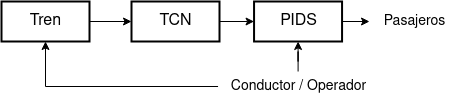
\includegraphics[width=0.66\textwidth]{./Figures/diagTrenTcnPids.png}
	\caption{Diagrama del sistema Tren-TCN-PIDS.}
	\label{fig:diagTrenTcnPids}
\end{figure}

La red TCN define una comunicación estándar usando dos buses jerárquicos llamados WTB (Wire Train Bus) y MVB (Multifunction Vehicle Bus). El sistema PIDS se interconecta al bus de datos MVB, como se indica en el diagrama de la figura \ref{fig:diagTcnPidsBuusesWtbMvb}.\\


\begin{figure}[ht]
	\centering
	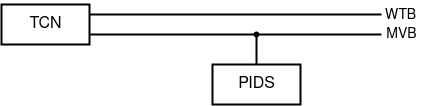
\includegraphics[width=0.66\textwidth]{./Figures/diagTcnPidsBusesWtbMvb.png}
	\caption{Diagrama de interconexión TCN-PIDS}
	\label{fig:diagTcnPidsBuusesWtbMvb}
\end{figure}

El sistema PIDS tiene un bus de comunicación propio a través de una red RS485. Uno de los componentes de esta red es el módulo SCU, al cual se conectan distintos dispositivos como los display LED, los mapas de recorrido LED, las cámaras y parlantes, tal como se indica en la figura 	\ref{fig:diagPidsScuDevices}.\\


\begin{figure}[ht]
	\centering
	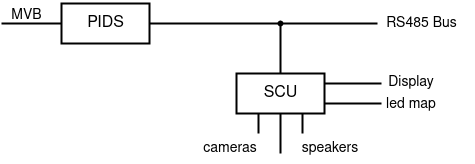
\includegraphics[width=0.66\textwidth]{./Figures/diagPidsScuDevices.png}
	\caption{Diagrama del módulo SCU en la red PIDS.}
	\label{fig:diagPidsScuDevices}
\end{figure}

Al módulo SCU se conectan las unidades IDU, que corresponden a los display LED de salón. Cada unidad IDU contiene un driver y el arreglo de módulos de matriz led que conforman el display. En la figura \ref{fig:diagScuDriverDisplay} se representan estos bloques funcionales.\\


\begin{figure}[ht]
	\centering
	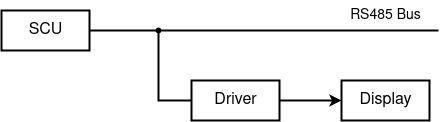
\includegraphics[width=0.66\textwidth]{./Figures/diagScuDriverDisplay.png}
	\caption{Diagrama de bloques del sistema SCU, placa de control y carteles LED de salón.}
	\label{fig:diagScuDriverDisplay}
\end{figure}

El alcance del sistema desarrollado en este trabajo cubre la funcionalidad de este conjunto de bloques Driver + Display, que en la nomenclatura del sistema PIDS existente corresponde a los módulos IDU. Existen dos unidades de estos módulos por cada salón o coche.\\

Muchas de las formaciones de SOFSE disponen de siete coches, por lo que se tiene un mínimo de catorce unidades IDU (dos por salón) más dos displays externos adicionales para el frente y contrafrente del tren que indican las estaciones cabecera del recorrido. Esto resulta en un total de al menos dieciséis unidades de control de display por cada tren. Teniendo en cuenta las formaciones operativas de las líneas Mitre, Sarmiento y Roca del Área Metropolitana de Buenos Aires (AMBA), se puede estimar alrededor de treinta trenes operando en simultáneo, lo que resulta en aproximadamente 500 unidades de displays operando en vivo. El impacto que puede tener el aporte de este trabajo estará directamente relacionado con la operación de Trenes Argentinos y definitivamente puede contribuir a la extensión de la vida útil de los trenes.\\

\subsection{Diseño}
La propuesta de diseño busca cubrir las funcionalidades del bloque de control del display LED. El display LED es una unidad que se puede adquirir comercialmente. Sin embargo el driver para la red PIDS es una solución propietaria del fabricante y es la que se busca reemplazar con este desarrollo.\\

En la figura \ref{fig:diagVistaReDisenhoEduCIAA} se presenta un diagrama de bloques del sistema de control propuesto. Este controlador usa comunicación serie a través de interfaces UART-RS485 y UART-USB. La UART es un periférico del microcontrolador de la plataforma CIAA. La alimentación de la CIAA difiere de aquella existente en la red RS485, por lo que también es necesario un bloque de conversión DC-DC para garantizar compatibilidad eléctrica. La comunicación con el display se realiza a través de un adaptador, que consiste básicamente en un puerto de entrada-salida.\\


\begin{figure}[ht]
	\centering
	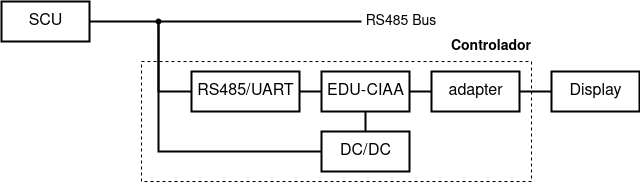
\includegraphics[width=0.75\textwidth]{./Figures/diagVistaReDisenhoEduCIAA.png}
	\caption{Diagrama de bloques del controlador propuesto.}
	\label{fig:diagVistaReDisenhoEduCIAA}
\end{figure}

A nivel lógico, el sistema que se propone consiste en cuatro objetos activos que interactúan entre sí, tal como se indica en la figura \ref{fig:diagVistaDisenho}. 

\begin{figure}[ht]
	\centering
	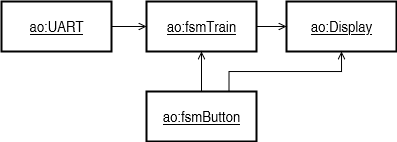
\includegraphics[width=1\textwidth]{./Figures/diagVistaDisenho.png}
	\caption{Vista estructural del sistema propuesto.}
	\label{fig:diagVistaDisenho}
\end{figure}

El objeto activo UART es el encargado de recibir e interpretar las tramas de datos que viajan por la red RS485 del bus de datos del SCU. El objeto activo Button es el control manual del operador para accionar el sistema. El objeto activo PIDS es una máquina de estados que representa el estado del tren y es el que contiene los mensajes y nombres de las estaciones. El objeto activo DisplayLed es el encargado de codificar los mensajes en el formato correspondiente a la matriz led del display. El prefijo "ao:" y el subrayado denotan objecto activo.\\

Esta vista estructural del sistema plantea la interacción entre componentes e indica su dependencia funcional. El diseño modular permite hacer cambios en los componentes de forma independiente. Por ejemplo se podrían reemplazar los mensajes al pasajero en el objeto PIDS sin afectar el resto del sistema, o bien reemplazar la lógica de control del display led si fuera necesario cambiar el hardware de control modificando únicamente el objeto DisplayLed.\\


\section{Implementación}
En este trabajo se implementa un sistema embebido usando el lenguaje de programación C y el sistema operativo de tiempo real freeRTOS. La plataforma de hardware utilizada es la CIAA-EDU-NXP, que dispone de un microcontrolador LPC4337 de la companía NXP (\citep{NXPLPC4337}), con una arquitectura de 32 bits ARM Cortex-M4/M0. El firmware se desarrolló utilizando también la \textit{SAPI} y el \textit{firmwarev3} \citep{firmwarev3} como capa de abstracción de hardware. Esta API es una interfaz para usar las funciones de la biblioteca CMSIS del fabricante del microcontrlador. Esta API es parte fundamental del proyecto CIAA.\\
 
En el diseño del sistema se desarrollaron plantillas para implementar patrones de software como máquinas de estado y objetos activos. Con las plantillas se facilita la documentación, testing, mantenimiento y escalabilidad. Estos fueron aspectos de calidad de software que se buscó satisfacer desde el diseño. Se describen los lineamientos y fragmentos de código principales de estas plantillas en la sección de patrones de software. \\

La implementación de los objetos activos del sistema se describe en la sección de componentes de sistema. Se mencionan los atributos principales de la solución y se documentan las vistas de interacción entre componentes. La implementación del controlador del diplay led tiene una sección a nivel de detalle para mayor comprensión. El firmware busca ser portable a aquellas versiones de hardware de display de matriz led compatibles con el conjunto de chips 74HC245, 74HC595 y 74HC138 o sistemas digitales equivalentes. \\



\subsection{Organización del código fuente}
La organización del código fuente que conforma el sistema embebido de este trabajo se describe en el siguiente árbol de archivos:

\begin{lstlisting}[
	language=Bash, 
	backgroundcolor=\color{mygray},
	]
AppRTOS
|-- config.mk
|-- inc
|   |-- common.h
|   |-- displayLed.h
|   |-- FreeRTOSConfig.h
|   |-- ISR_GPIO.h
|   |-- ISR_UART.h
|   |-- main.h
|   |-- modulePanelDisplay.h
|   |-- portmap.h
|   |-- statemachine_AB.h
|   |-- statemachine_button.h
|   |-- statemachine_displayLed.h
|   |-- statemachine_PIDS.h
|   |-- statemachine_UART.h
|   `-- userTasks.h
|-- LICENSE.txt
`-- src
    |-- displayLed.c
    |-- ISR_GPIO.c
    |-- ISR_UART.c
    |-- main.c
    |-- statemachine_AB.c
    |-- statemachine_button.c
    |-- statemachine_displayLed.c
    |-- statemachine_PIDS.c
    |-- statemachine_UART.c
    `-- userTasks.c
\end{lstlisting}

Se pueden observar dos directorios principales: \textit{inc} y \textit{src}. En \textit{inc} se incluyen los archivos de encabezados y en \textit{src} los archivos de código ejecutable. Existe un archivo principal o \textit{main} que es el que instancia las secuencias de incialización, recursos y tareas del sistema operativo. Las tareas, que incluyen a los objetos activos y procesos del sistema, se implementan en los archivos \textit{userTasks}. Luego, para cada implementación de objeto activo existe una máquina de estados asociada en un archivo de encabezados y un archivo ejecutable con el prefijo \textit{statemachine}. Finalmente los archivos con el prefijo \textit{ISR} corresponden a las rutinas de interrupción. Como cada máquina de estado utiliza recursos del sistema operativo, se ha creado un archivo common.h que declara aquellos recursos como colas, handlers y semáforos que se utilizan entre tareas para comunicación interprocesos.\\

Esta organización permite encapsulamiento y modularidad de los componentes del sistema. De esta manera se facilita el mantenimiento y con el uso de las mismas reglas de diseño se facilita la escalabilidad.\\

\subsection{Uso de recursos en RTOS}

En este desarrollo se utiliza freeRTOS, una versión en C de un kernel de sistema operativo de tiempo real. La implementación se basa en la inclusión de los archivos de cabecera FreeRTOS.h y FreeRTOSConfig.h. Esta implementación ha sido validada en arquitecturas ARM Cortex-M4, en particular en la plataforma EDU-CIAA. 

En todos los casos que fue posible se utilizaron semáforos, colas y mutex para organizar y proteger el uso compartido de recursos. El caso de uso típico de \textit{mutex} es la interacción de distintas tareas con la misma interfaz UART-USB para imprimir mensajes por pantalla. En el código fuente de cada objeto implementado se utiliza la siguiente plantilla para proteger el recurso evitando accesos múltiples y posibilidad de deadlock:\\

\begin{lstlisting}[
	language=C, 
	backgroundcolor=\color{mygray},
	]
if (pdTRUE == xSemaphoreTake( xMutexUART, portMAX_DELAY)){
   vPrintString("Task AB is running.\r\n");
   xSemaphoreGive(xMutexUART);
}
\end{lstlisting}

Las colas, \textit{Queue}, se utilizan principalmente para comunicar eventos entre objetos activos. En todos los casos se referencian con handlers usando la nomenclatura con prefijo \textit{queueHandle}. En el siguiente fragmento de código se muestra un ejemplo, exibiendo los mecanismos de control de errores usados. \\

\begin{lstlisting}[
	language=C, 
	backgroundcolor=\color{mygray},
	]
queueHandle_button = xQueueCreate(QUEUE_MAX_LENGTH, sizeof(eSystemEvent_button));
if (queueHandle_button == NULL){
    perror("Error creating queue");
    return 1;
}
\end{lstlisting}


Todas las tareas y recursos del sistema operativo se han protegido contra errores informando al usuario ante fallas en la instanciación previas al inicio del scheduler.

\begin{lstlisting}[
	language=C, 
	backgroundcolor=\color{mygray},
	]
if( xTaskCreate( vTaskReadSerial, "Serial Comm reading task", 
    configMINIMAL_STACK_SIZE*4, NULL, tskIDLE_PRIORITY+2, &xTaskReadSerialHandler) 
    == pdFAIL ) {
    perror("Error creating task");
}
\end{lstlisting}

Se utilizan también punteros de tipo \textit{xTaskHandle}para referenciar las tareas del sistema operativo. Este tipo de referencias es de especial utilidad a la hora de eliminar tareas de forma dinámica en tiempo de ejecución. También es posible usar estas referencias para comunicación entre tareas.\\

El uso de \textit{Timers} por software fue el preferido en aquellos casos que su uso facilita el mantenimiento, legibilidad y comprensión de la implementación. La plantilla desarrollada para la creación de timers se presenta en el siguiente fragmento de código.

\begin{lstlisting}[
	language=C, 
	backgroundcolor=\color{mygray},
	]
void timerCallback_displayLed(TimerHandle_t xTimerDisplayHandle){

   if (pdTRUE == xSemaphoreTake( xMutexUART, portMAX_DELAY)){
      printf("Timer display led is running.\r\n");
      xSemaphoreGive(xMutexUART);
   }

   eSystemEvent_displayLed  displayLed_timer_event = evDisplayled_timeout;
   
   if(xQueueSend(queueHandle_displayLed, &displayLed_timer_event, 0U)!=pdPASS){
         perror("Error sending data to the queueHandle_displayLed\r\n");
   }
}

\end{lstlisting}

Se procuró tener especial cuidado de superposición o competición del reloj del sistema operativo entre tareas. Distintos componentes pueden tener requisitos temporales que compiten entre si por prioridad del scheduler. Se verá en detalle la implementación del display Led como ejemplo que puede competir con el arribo de mensajes por la interfaz UART.\\

Las rutinas de interrupción por hardware o \textit{ISR} se utilizan cuando se requiere respuesta inmediata, como al accionar manualmente un interruptor o bien al recibir mensajes o señales eléctricas desde el bus de datos del tren. La implementación elegida para el uso de interrupciones se representa en el diagrama de secuencia de la figura \ref{fig:ISR}. \\

\begin{figure}[ht]
	\centering
	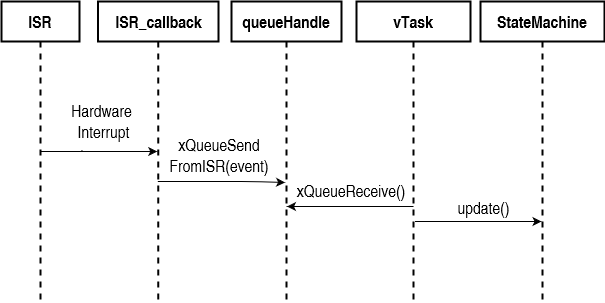
\includegraphics[width=1\textwidth]{./Figures/ISRcallback.png}
	\caption{Diagrama de secuencia que representa la interacción entre componentes del sistema operativo cuando se dispara una interrupción o ISR.}
	\label{fig:ISR}
\end{figure}

El recurso de hardware que genera interrupciones (ISR) llama a una función callback (\textit{ISR callback}) que sólo se encarga de entregar un mensaje de evento al sistema, no tiene lógica implementada, sólo avisa al sistema que hay una interrupción que atender. El evento se comunica a través de una cola, recurso elegido como interfaz de mensajes de los objetos activos. La cola es atendida por una tarea de sistema (vTask) que resuelve el código de ejecución. Esta tarea normalmente implementa un objeto activo que actualiza una máquina de estado.\\

Si bien puede llamar la atención la complejidad del mecanismo de atención de una interrupción, este patrón basado en objeto activo permite desacoplar la invocación y la ejecución en una máquina de estados. El objeto activo es una técnica de concurrencia muy utilizada por la ventaja de separar en hilos independientes la invocación de funciones (eventos) de las funciones de ejecución. Con esto, la posibilidad de atender múltiples eventos en simultáneo, sin esperar a que se procese cada evento secuencialmente. Se logra paralelismo, atomicidad en el callback de la interrupción, muy baja latencia, y se mantiene consistencia en el uso de objetos activos siguiendo los lineamientos de la arquitectura orientada a eventos.\\


Por último se menciona el uso de Memoria dinámica. El sistema tiene una interfaz de comunicación UART que a priori recibirá mensajes de largo variable y desconocido. Por lo tanto, el uso de buffers dinámicos para el almacenamiento y procesamiento de datos fue preferido. Para utilizar memoria dinámica se usan las funciones memset(), pvPortMalloc(), memcpy() y vPortFree() a través de dos instancias de ejecución: una de recepción y almacenamiento de datos, y otra de ejecución y liberación de memoria. En el siguiente fragmento de código se explica este uso de funciones con dos tareas reader y writer.


\begin{lstlisting}[
	language=C, 
	backgroundcolor=\color{mygray},
	]
void vTaskReader(void *parameters) {
   // Clear whole buffer
   memset(buf, 0, buf_len);
   // Loop forever
   while (true) {
   // Read from UART
      uint8_t c_data=0;
      if (uartReadByte( UART_USB, &c_data ) == true ){
      // Store to buffer if not over buffer limit  
         if (idx < buf_len - 1){
            buf[idx] = c_data;
            idx++;
         }
         // Create a message ending string with null
         if (c_data == '\n') {
            buf[idx - 1] = '\0';
            // Allocate memory and copy message. 
            if (msg_flag == 0) {
               msg_ptr = (char *)pvPortMalloc(idx * sizeof(char));
               if (msg_ptr==NULL){
                  if (pdTRUE == xSemaphoreTake( xMutexUART, portMAX_DELAY)){
                     printf("Buffer out of memory\r\n");
                     xSemaphoreGive(xMutexUART);
                  }
               }
               // Copy message
               memcpy(msg_ptr, buf, idx);
               // Notify other task that message is ready
               msg_flag = 1;
            }
            // Reset buffer and index
            memset(buf, 0, buf_len);
            idx = 0;
         }
      }
   }
}     

void vTaskWriter(void *parameters) {
   if (uart_msg_flag == true) {
      // Print the message in the buffer 
      if (pdTRUE == xSemaphoreTake( xMutexUART, portMAX_DELAY)){
        printf("%s\r\n", uart_msg_ptr);
        xSemaphoreGive(xMutexUART);
      }
      // Free the memory block  
      vPortFree(uart_msg_ptr);  
      uart_msg_ptr  = NULL;
   }
}

\end{lstlisting}

Como se puede observar, cuando se recibe un caracter por la interfaz UART se copia el mismo en el buffer siempre y cuando no esté lleno. Cuando el buffer se completa, se pide memoria y se copia el mensaje usando un puntero al bloque de memoria asignado. Luego la tarea de ejecución lee el mensaje de ese puntero a memoria o bien lo procesa para invocar otra función.\\


\subsection{Patrones de software}
En este desarrollo se ha hecho uso extensivo de los patrones máquina de estado, objeto activo, pipeline, observ and react, y superciclo. Se presenta en detalle el formato de plantillas desarrollado en C para freeRTOS para los patrones de máquinas de estado y de objeto activo. \\

\subsubsection{Máquinas de estado}
El desarrollo de la arquitectura orientada a eventos propuesta se basa en la interacción de máquinas de estado usando objetos activos. En este trabajo las máquinas de estado se implementan sistemáticamente en C con el siguiente procedimiento paso a paso:

\begin{enumerate}
\item Representación de los estados y eventos con diagrama de estados.
\begin{figure}[ht]
	\centering
	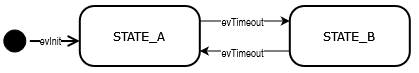
\includegraphics[width=0.66\textwidth]{./Figures/statemachineAB.png}
	\caption{Diagrama de la máquina de estados AB ejemplo.}
	\label{fig:fsmAB}
\end{figure}

\item Definición de los estados, usando tipo enumerativo definido con el prefijo \textit{eSystemState}:

\begin{lstlisting}[
	language=C, 
	backgroundcolor=\color{mygray},
	]
typedef enum{
    
    STATE_INIT,
	STATE_A,
	STATE_B

} eSystemState;
\end{lstlisting}

\item Definición de los eventos. Los eventos representan transiciones entre estados con un tipo enumerativo definido con el prefijo \textit{eSystemEvent}:

\begin{lstlisting}[
	language=C, 
	backgroundcolor=\color{mygray},
	]
typedef enum{

	evInit,
	evTimeout

} eSystemEvent;
\end{lstlisting}

\item Definición de un tipo puntero a función usando el prefijo \textit{*pfEventHandler()} para designar los handlers específicos:

\begin{lstlisting}[
	language=C, 
	backgroundcolor=\color{mygray},
	]
typedef eSystemState (*pfEventHandler)(void);
\end{lstlisting}

\item Definición de una estructura para la máquina de estados definiendo un tipo \textit{sStateMachine}. Esta estructura debe incluir una variable estado (eSystemState), una variable evento (eSystemEvent) y un puntero a función (pfEventHandler). El puntero a función será una instancia de handler específico que maneje las transiciones entre estados. 

\begin{lstlisting}[
	language=C, 
	backgroundcolor=\color{mygray},
	]
typedef struct{

	eSystemState  	fsmState;
	eSystemEvent  	fsmEvent;
	pfEventHandler	fsmHandler;

} sStateMachine;
\end{lstlisting}

\item Definición de los handlers a implementar para el manejo de ejecución y transiciones entre estados.

\begin{lstlisting}[
	language=C, 
	backgroundcolor=\color{mygray},
	]
eSystemState 	InitHandler(void);
eSystemState 	AHandler(void);
eSystemState 	BHandler(void);
\end{lstlisting}

\item Instanciación de la máquina de estados como un arreglo de estructuras usando el prefijo \textit{sStateMachine\_}. Para el ejemplo de la máquina AB la instancia de arreglo de estructuras sería la siguiente:

\begin{lstlisting}[
	language=C, 
	backgroundcolor=\color{mygray},
	]
sStateMachine_AB fsmMachineAB [] = 
{
	{STATE_INIT_AB, evInit_AB, InitHandler_AB},
	{STATE_A, evTimeout, AHandler},
	{STATE_B, evTimeout, BHandler}
};
\end{lstlisting}

En esta definición habrá un handler en el momento de inicialización (initHandler), un handler específico para cada estado.

\item Escribir el código ejecutable de los handlers. Una implementación  modo de ejemplo se presenta en el siguiente fragmento de código:

\begin{lstlisting}[
	language=C, 
	backgroundcolor=\color{mygray},
	]
eSystemState 	InitHandler(void){ 
	printf("State Machine Init...\n");
	return STATE_A; 
}

eSystemState 	AHandler(void){ 
	printf("State Machine State A\n");
	return STATE_B; 
}

eSystemState 	BHandler(void){ 
	printf("State Machine State B\n");
	return STATE_A; 
}
\end{lstlisting}
\end{enumerate}


Se debe notar que para este ejemplo cada transición de estados se ejecutará por el evento \textit{evTimeout}. La máquina inicia y se define en el estado STATE\_A y luego alterna entre STATE\_A y STATE\_B por cada evento de timeout.

De esta manera queda desacoplada la implentación de los handlers del resto de la estructura de la máquina de estados, logrando portabilidad, escala y modularidad. Los handlers serán funciones que se implementan con el sufijo Handler() y que por definición tienen un solo argumento de tipo void.

Con esta técnica de desacoplamiento, se implementan dos archivos por cada máquina de estado : uno de encabezados (stateMachine.h) con las definiciones y otro con la implementación (stateMachine.c) de los handlers.




\subsubsection{Objeto Activo}
	
Los objetos activos se implementan en esta aplicación como tareas de freeRTOS con dos superciclos anidados de tipo \textit{while(true)}, como se muestra en el siguiente fragmento de código: 

\begin{lstlisting}[
	language=C, 
	backgroundcolor=\color{mygray},
	]
void vTaskAB(void *xTimerHandle)
{
   (void)xTimerHandle;

   // Task successful creation message
   if (pdTRUE == xSemaphoreTake( xMutexUART, portMAX_DELAY)){
      printf("Task AB is running.\r\n");
      xSemaphoreGive(xMutexUART);
   }

   while(true){
      
      // State machine init
      eSystemEvent_AB newEvent	=	evInit_AB;
      eSystemState_AB nextState	=	STATE_INIT_AB;
      fsmMachineAB[nextState].fsmEvent = newEvent; 
      nextState = (*fsmMachineAB[nextState].fsmHandler)();

      // Active object
      while(true){
        if( pdPASS == xQueueReceive(queueHandle_AB, &newEvent, portMAX_DELAY)){
            fsmMachineAB[nextState].fsmEvent = newEvent; 
            nextState = (*fsmMachineAB[nextState].fsmHandler)();
         }
      }
   }
}
\end{lstlisting}

Notar que el primer ciclo while() es el que corresponde al funcionamiento normal de una tarea o proceso de RTOS. En este caso es el encargado de inicializar la máquina de estados asociada al objeto activo. El superciclo while() de la línea 20 se encarga de bloquear la tarea hasta que se reciba un evento por la interfaz (cola de eventos). La interfaz del objeto activo es una cola FIFO con la función de sistema xQueueReceive() (línea 21). Si se recibe un evento, entonces se actualiza el estado de la máquina instanciando el handler que corresponda, como se observa en la línea 25. El diagrama de la figura \ref{fig:AOfsmAB} representa el objeto activo detallado. 

\begin{figure}[ht]
	\centering
	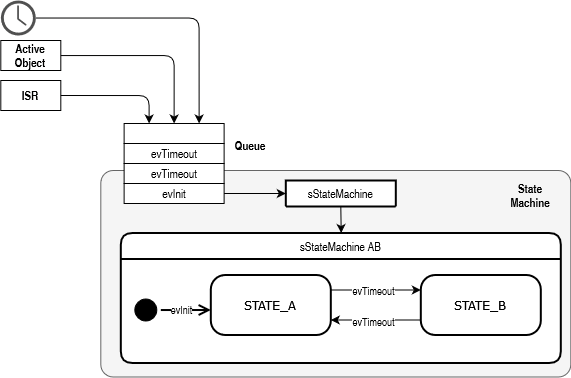
\includegraphics[width=0.85\textwidth]{./Figures/AOstatemachineAB.png}
	\caption{Diagrama del objeto activo de la máquina de estados AB ejemplo.}
	\label{fig:AOfsmAB}
\end{figure}

En este caso la tarea de sistema recibe una referencia a un timer (xTimerHandle) que genera eventos de timeout y los encola en la interfaz del objeto activo (Queue). Con la misma interfaz, los eventos podrían ser generados también por otros objetos activos o por rutinas de interrupción. Los mensajes en cola se reciben en la tarea de sistema que actualiza la máquina de estados.\\

\subsection{Componentes del sistema}

En esta sección se describen los componentes principales de la solución representada con el diagrama estructural de la figura \ref{fig:diagVistaDisenho}. En la figura \ref{fig:diagramaSecuenciaSistema} se presentan las interacciones entre componentes en forma de secuencia para los distintos casos de uso. Los cuatro objetos activos utilizados son:\\
\begin{itemize}
\item \textbf{UART}: objeto activo que sirve de interfaz de comunicación con la red RS485 del sistema PIDS. Se encarga de recibir los mensajes de la red, identificarlos y enviarlos al objeto PIDS.
\item \textbf{PIDS}: objeto activo que contiene la lógica de procesamiento de señales del tren, los mensajes que se visualizan en pantalla y los trayectos disponibles. 
\item \textbf{displayLED}: objeto activo responsable de codificar los mensajes que vienen del PIDS para ser visualizados en un display de matriz led.
\item \textbf{Button}: objeto activo responsable de recibir accionamientos manuales del conductor del tren.
\end{itemize}

\begin{figure}[ht]
	\centering
	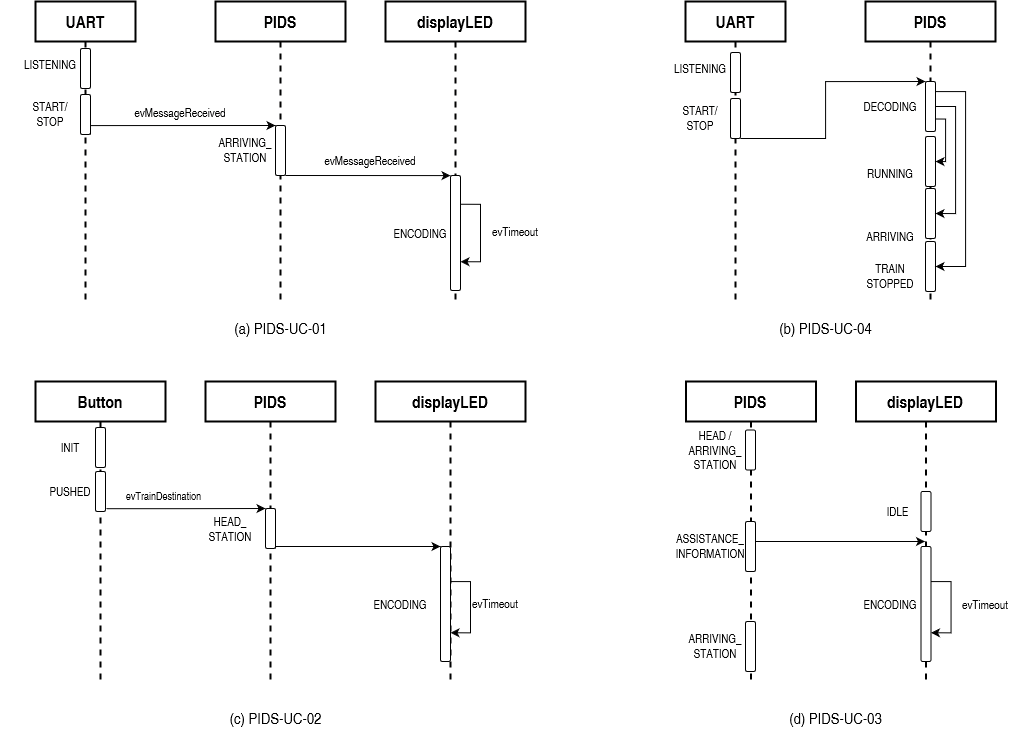
\includegraphics[width=1\textwidth]{../Figures/secuenciasSistema.png}
	\caption{(a)caso de uso de visualización de estación; (b) caso de uso de receptor de tramas;(c) caso de uso de elección de destino por accionamiento del conductor;(d) caso de uso de visualización de información de asistencia.}
	\label{fig:diagramaSecuenciaSistema}
\end{figure}


La organización del scheduler del sistema operativo se representa con el diagrama temporal de la figura \ref{fig:diagramasTemporales}. La base de este diagrama es el orden de prioridades de las tareas de objetos activos, los timers y los handlers de interrupciones que manejan los periféricos de hardware.\\

\subsubsection{UART}

En esta sección se describe la implementación del componente objeto activo UART (Universal Asynchronous Receiver Transmitter) del sistema. Este tipo de interfaz suele ser común en numerosas aplicaciones y abundan ejemplos utilizados para leer y escribir desde y hacia un periférico UART. El caso trivial es una aplicación "eco": todo lo que se recibe por la UART se vuelve a escribir y enviar por la UART. Sin embargo, la aplicación específica determina la lógica de procesamiento de mensajes. Por ejemplo si se recibe un caracter determinado, entonces se activa tal objeto; si se genera un evento en tal otro objeto, entonces se envía un mensaje de aviso. \\

En el sistema desarrollado, la UART es la interfaz de comunicación con el resto de la red PIDS. Esta debe procesar eventos que indican aceleración y desaceleración del tren. Los eventos se reciben codificados en tramas con formato específico, que a priori carecen de documentación. Como se verá en la sección de ensayos, se ha observado que las tramas normalmente tienen un encabezado (header), una carga de datos (payload), y un final de trama (trailer). Sin embargo, se ha observado también que los mensajes del tren pueden tener largo variable. El diseño de este componente se representa con el diagrama de la figura \ref{fig:diagfsmUART}.\\


\begin{figure}[ht]
	\centering
	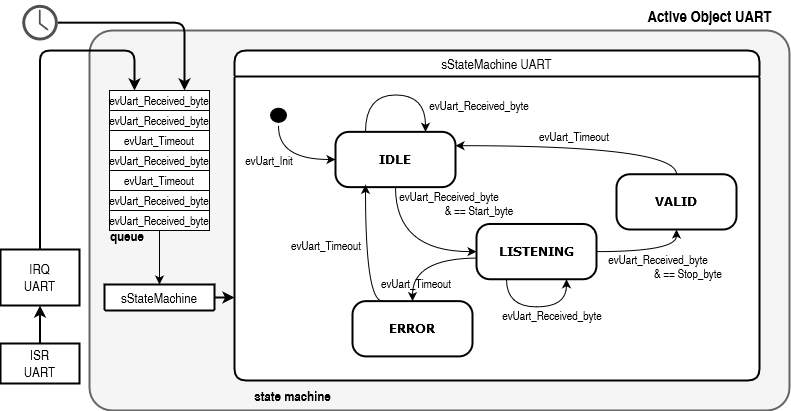
\includegraphics[width=1\textwidth]{./Figures/fsmUART3.png}
	\caption{Diagrama del objeto activo UART implementado.}
	\label{fig:diagfsmUART}
\end{figure}

El periférico UART es un componente de bajo nivel del microcontrolador que admite el control por interrupciones (ISR). Cada byte entrante genera una interrupción y de inmediato el handler IRQ\_UART envía un mensaje de actualización al objeto activo. Los eventos admitidos son:
\begin{itemize}
\item evUart\_Received\_byte para la recepción de un byte de datos; 
\item evUart\_Timeout, generado por un timer específico de control.\\
\end{itemize} 

La máquina de estados admite cuatro estados distintos:
\begin{itemize}
\item IDLE: estado inicial y de reposo.
\item LISTENING: estado generado al recibir el Header o inicio de trama.
\item VALID: estado generado al completar un mensaje con el Trailer o final de trama.
\item ERROR: estado alcanzado una vez generado un timeout en el estado listening.
\end{itemize}

El estado Listening es el core de la máquina de estados. El handler de ejecución permite guardar en memoria dinámica el contenido de un mensaje de largo variable una vez que se recibe un byte de inicio de trama.  El mensaje se completa cuando se recibe un byte de final de trama, que genera mediante timeout el evento de transición al estado Valid. La lógica que se plantea con este diseño es que una vez validada una trama de datos, se genere un evento de actualización hacia el componente externo PIDS.\\

De esta manera se diseñó un componente UART flexible, que permite cambiar los bytes de header y trailer y admite un buffer de largo variable usando memoria dinámica. \\

\subsubsection{Display LED}

El objetivo de esta sección es describir la solución implementada para el manejo de carteles de matriz led, su estructura, su forma de uso y cómo se debe modificar en caso de reutilización en otros sistemas.\\

Los carteles led de esta se basan en una tecnología de microcontrolador (MCU) y sistema digital. El MCU genera las señales de control y el sistema digital se encarga de codificar los datos del micro en señales eléctricas para prender leds de forma ordenada. Los display se componen de módulos de matriz led de 8x8. Estos módulos se direccionan por filas y columnas para  visualizar información. Los arreglos de estos módulos forman paneles, y estos últimos pueden ser direccionados por un grupo de señales de control. En la figura \ref{fig:diagDriverLED} se presenta el diagrama de bloques del sistema de control de los carteles de matriz led.\\


\begin{figure}[ht]
	\centering
	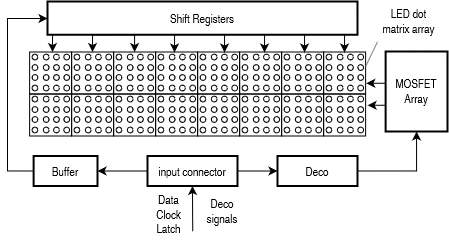
\includegraphics[width=1\textwidth]{./Figures/diagDriverLED.png}
	\caption{Diagrama de bloques del controlador de los carteles de matriz LED utilizados en esta implementación.}
	\label{fig:diagDriverLED}
\end{figure}

Las señales de control (data, clock, latch, deco) se generan en el MCU y se transmiten al circuito eléctrico del display led a través de un conector (CONN). Estas señales se direccionan eléctricamente usando buffers. Luego, hacia la izquierda, se transmiten las señales data, clock y latch, que envían los datos del mensaje codificado a un arreglo de Shift Registers. Estos últimos son los encargados de transmitir bit a bit los datos para las columnas de cada módulo que forman una fila completa del cartel. Una vez enviados todos los datos de una fila, se envía un pulso como señal de latch y se energiza la fila completa. Se repite la operación fila a fila escaneando todo el cartel a través de las señales del Deco, energizando cada fila a través de un arreglo de transistores MOSFET que mantienen la corriente necesaria para encender los leds. Este encendido por fila sucede durante un período de tiempo tal que toda la pantalla se pueda energizar en el orden de 20 a 50 veces por segundo para formar una imagen continua vista por el ojo humano.\\

\begin{figure}[ht]
	\centering
	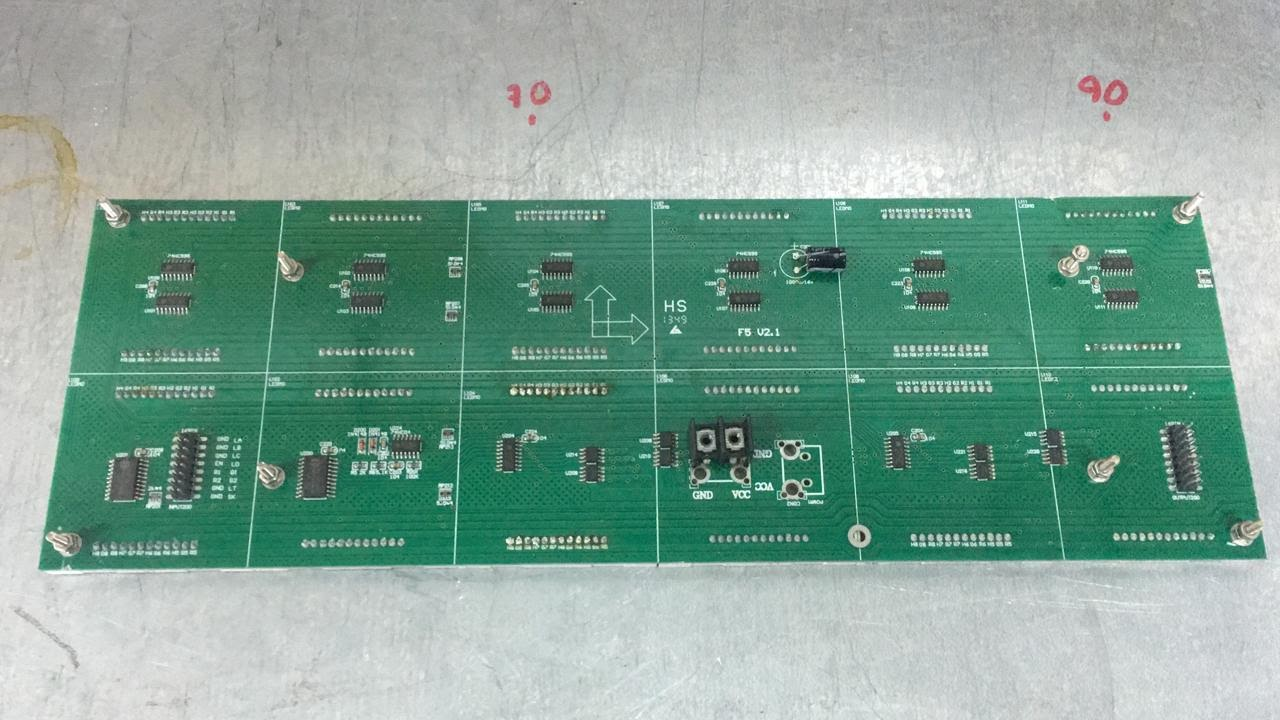
\includegraphics[width=1\textwidth]{./Figures/cartel2x6.jpeg}
	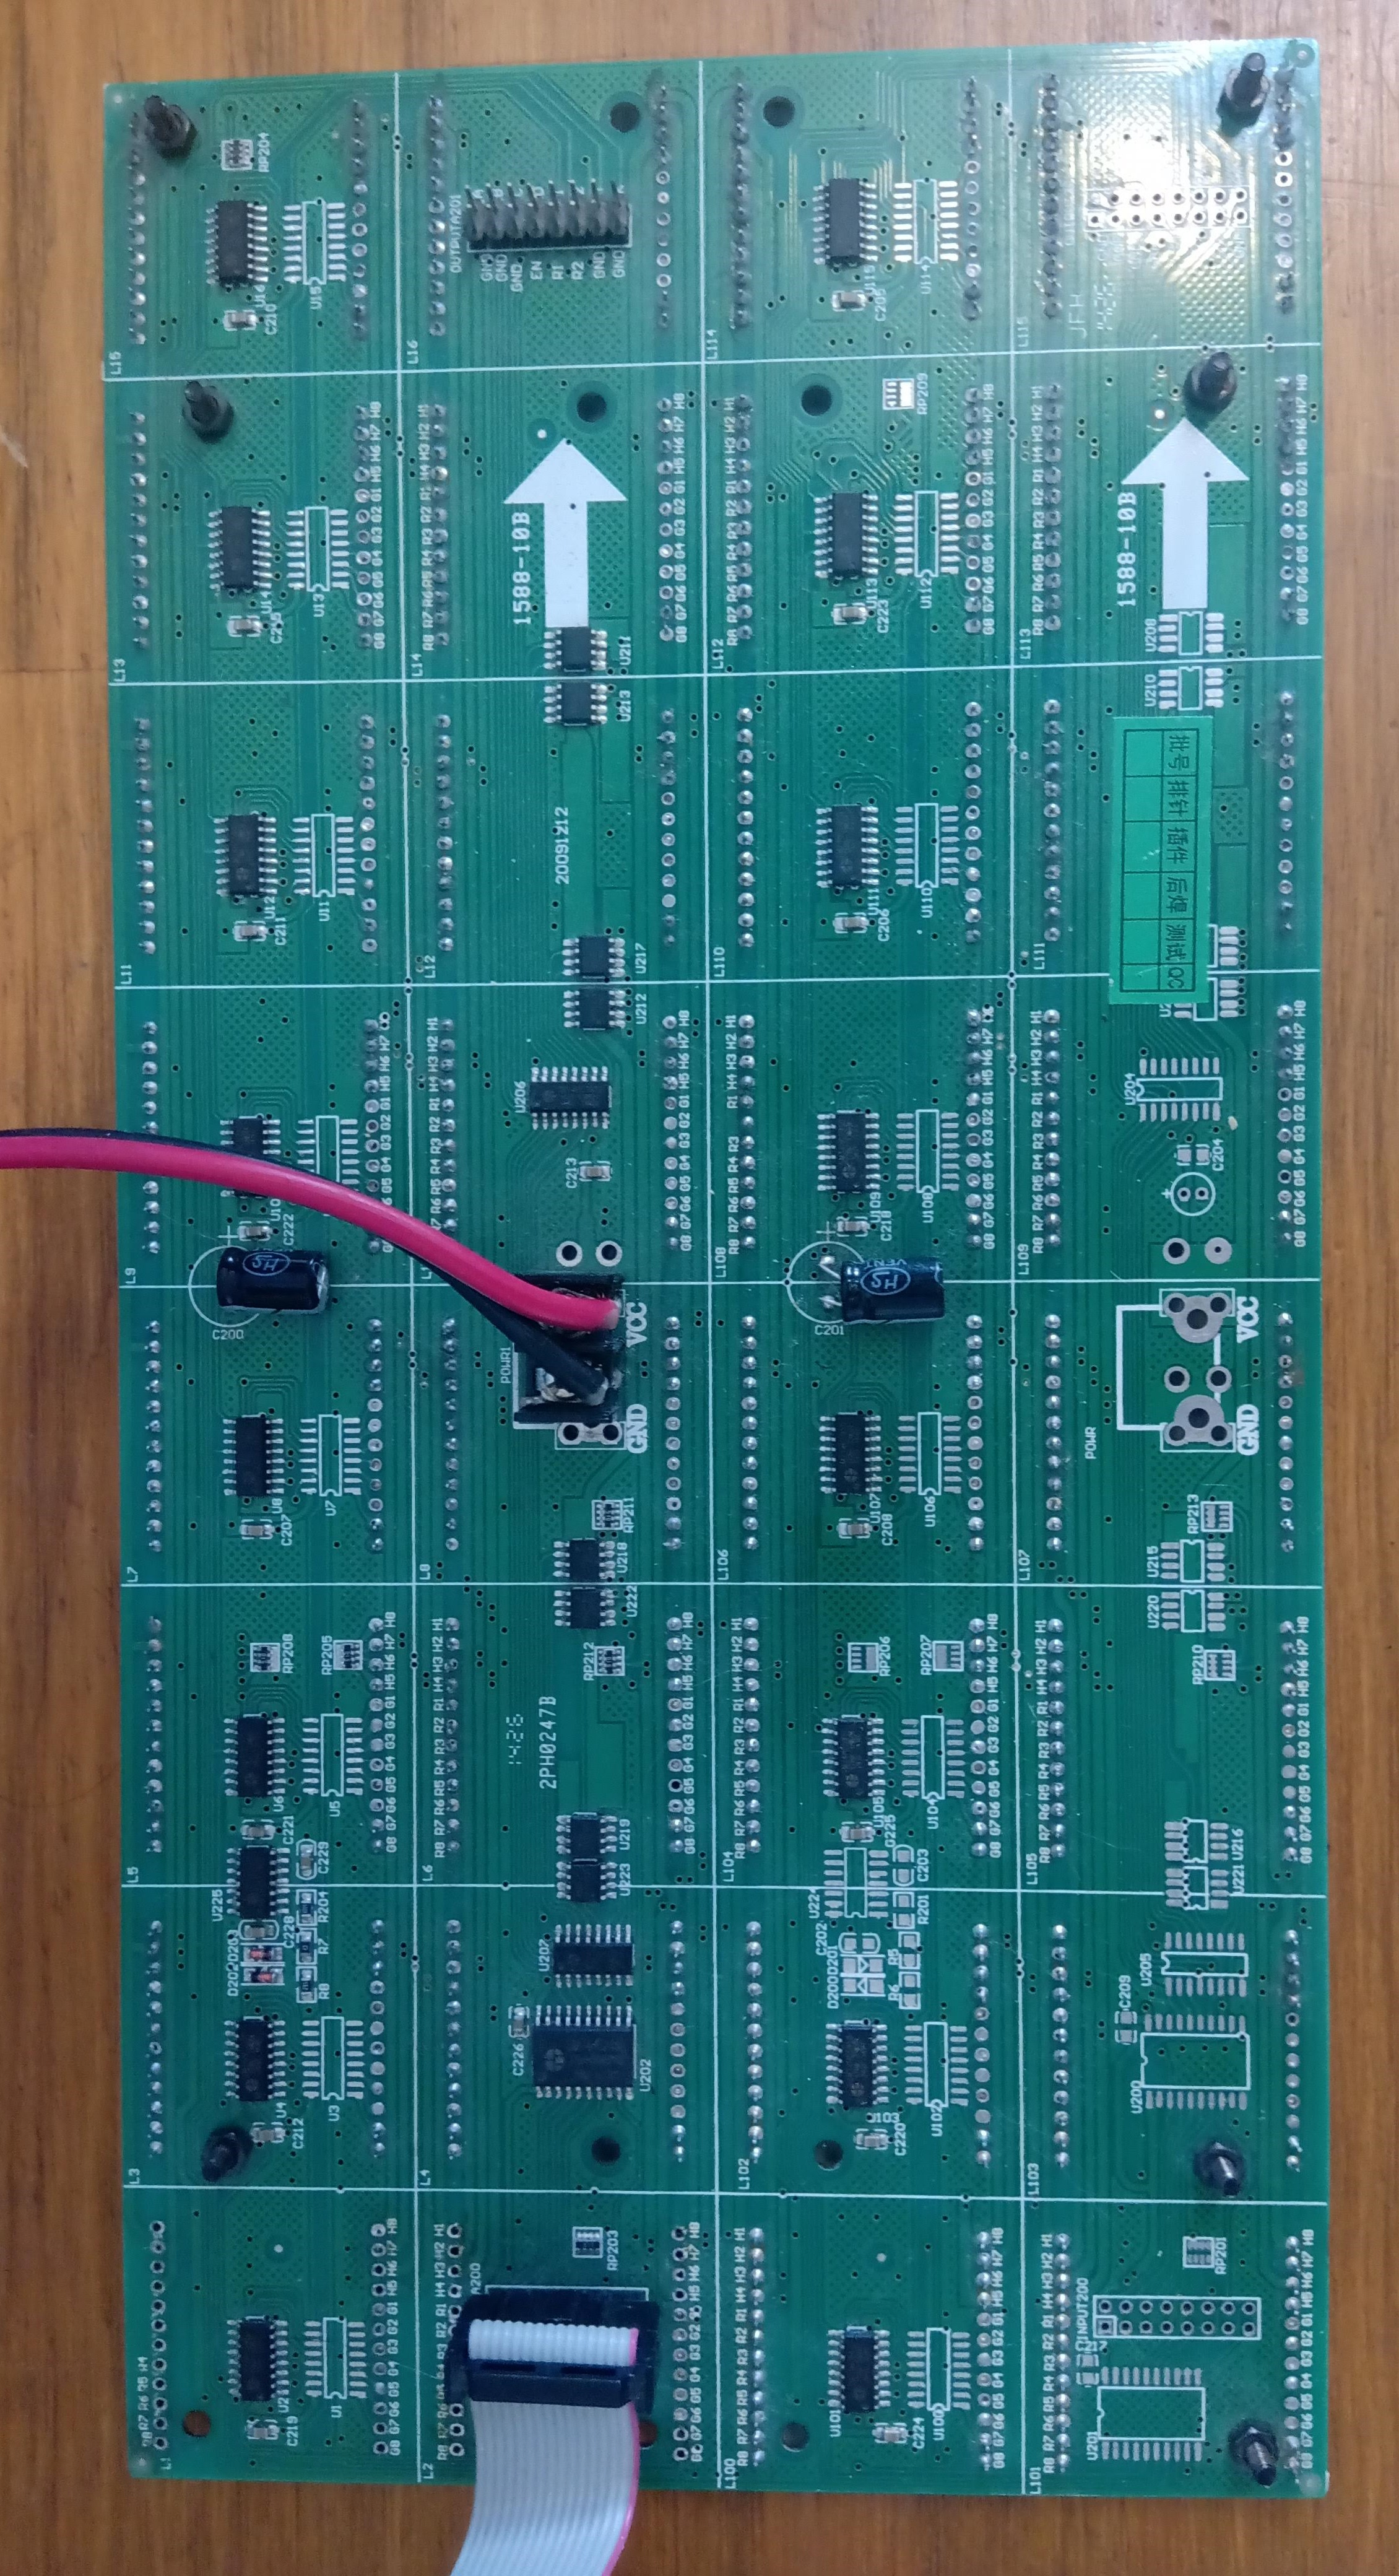
\includegraphics[width=0.75\textwidth, angle=270]{./Figures/cartel4x8.jpg}\\
	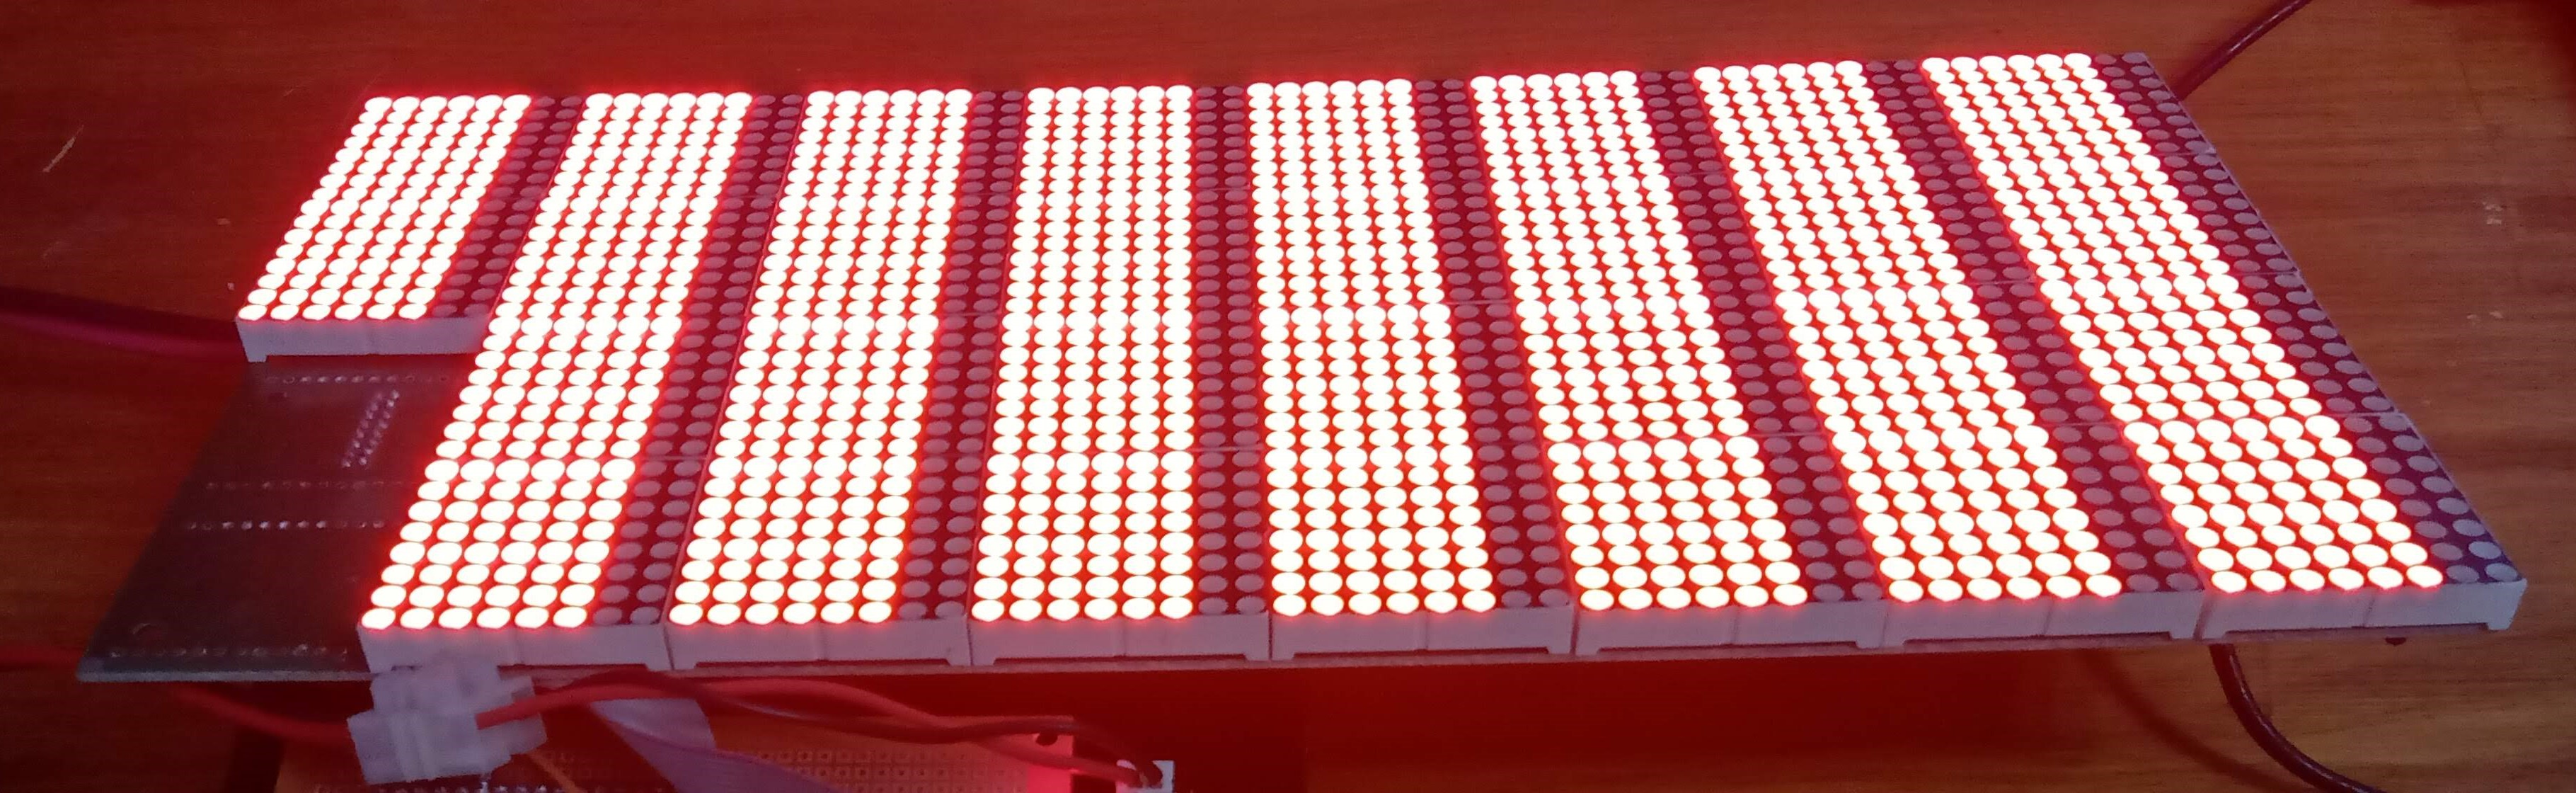
\includegraphics[width=1\textwidth]{./Figures/cartelLedON.jpg}\\
	\caption{Fotografías de placas de control de los carteles de matriz LED: (a) placa de 2x6 módulos; (b) placa de 4x8 módulos; (c) vista posterior de la placa de 4x8.}
	\label{fig:picsDriverLED}
\end{figure}

En el circuito esquemático de la figura \ref{fig:schDriverLED} se presenta el detalle de conexiones eléctricas entre bloques. Se puede observar que a la salida del conector de datos (CONN 2x8) hay dos buffers de la serie 74HC245D que direccionan las señales eléctricas a izquierda y derecha del arreglo de matrices led. A izquierda viajan las señales SER(data), SRCLK (Clock) y XXX (latch) al arreglo de Shift Registers de la serie 74HC595. Por la derecha se maneja la habilitación secuencial de las filas a través de un arreglo de decodificadores 3x8 de la serie 74HC138. Cada salida de los decodificadores se conecta a un driver de corriente en arreglo de transistores MOSFET FDS4953. Estos decodificadores cableados adecuadamente permiten manejar las 32 señales de un cartel de 4x8 módulos led. \\


\begin{figure}[ht]
	\centering
	%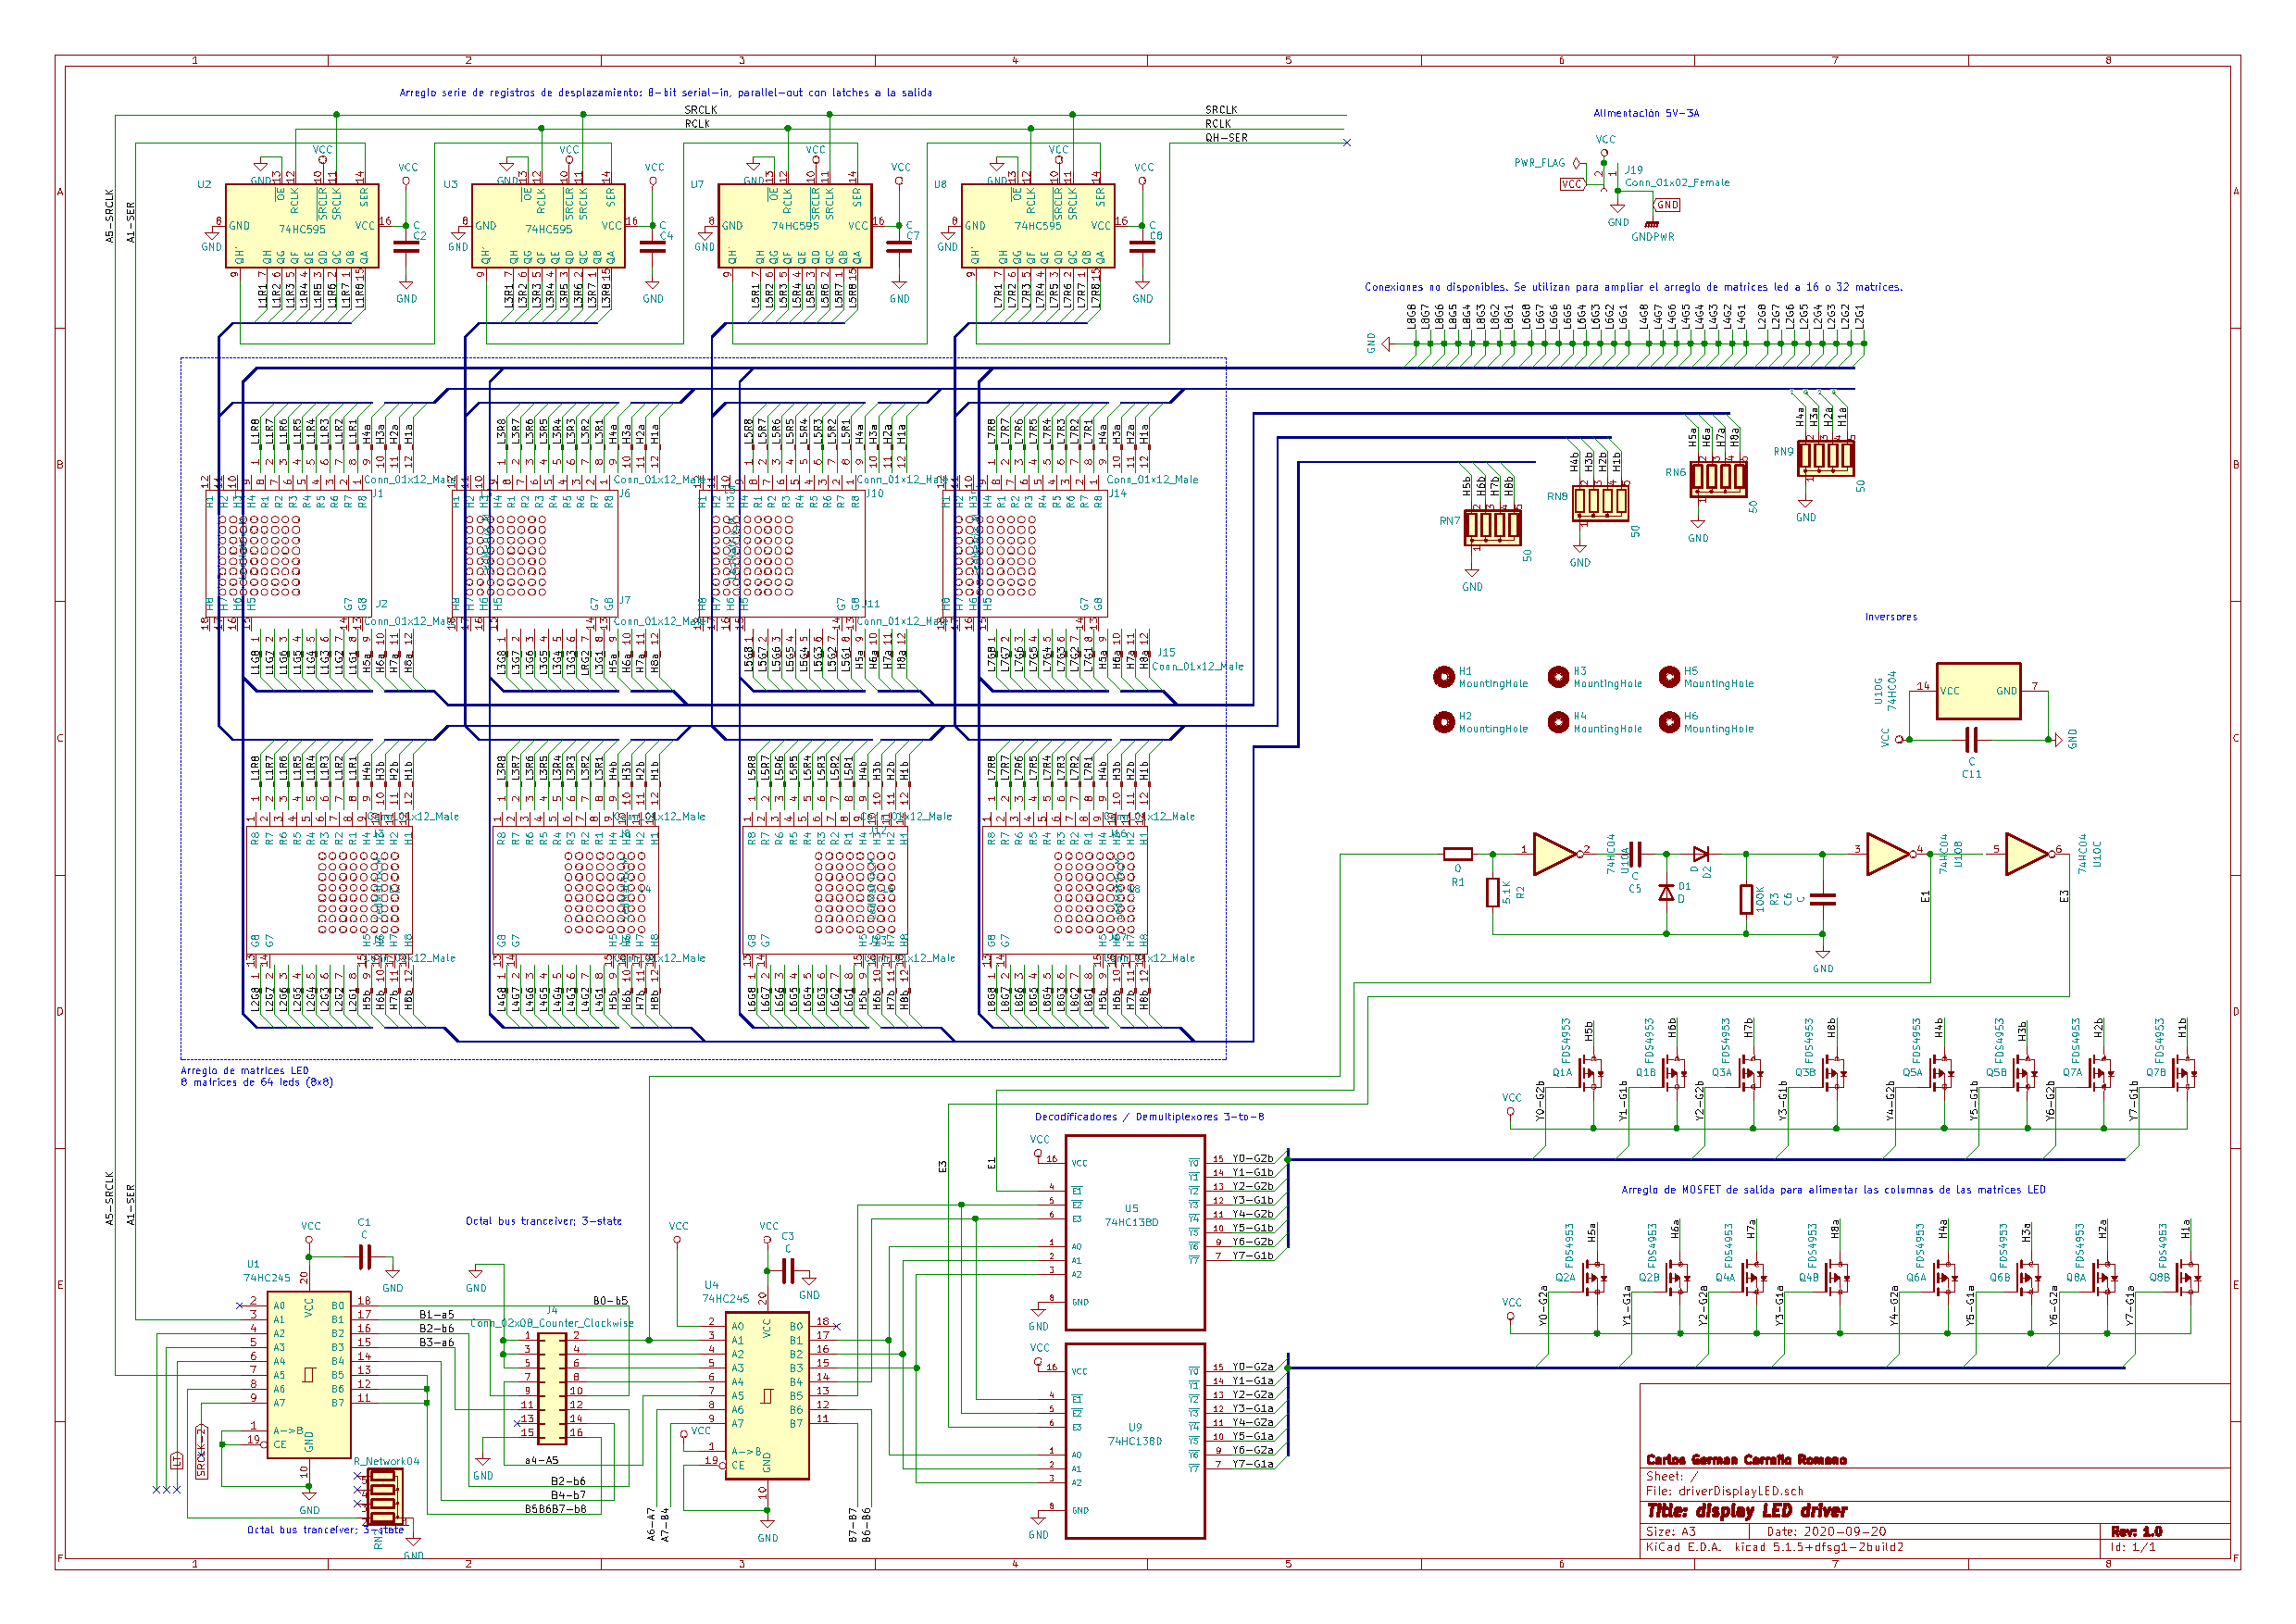
\includepdf[pages={1}, angle=90]{./Figures/output.driverLED.pdf}
	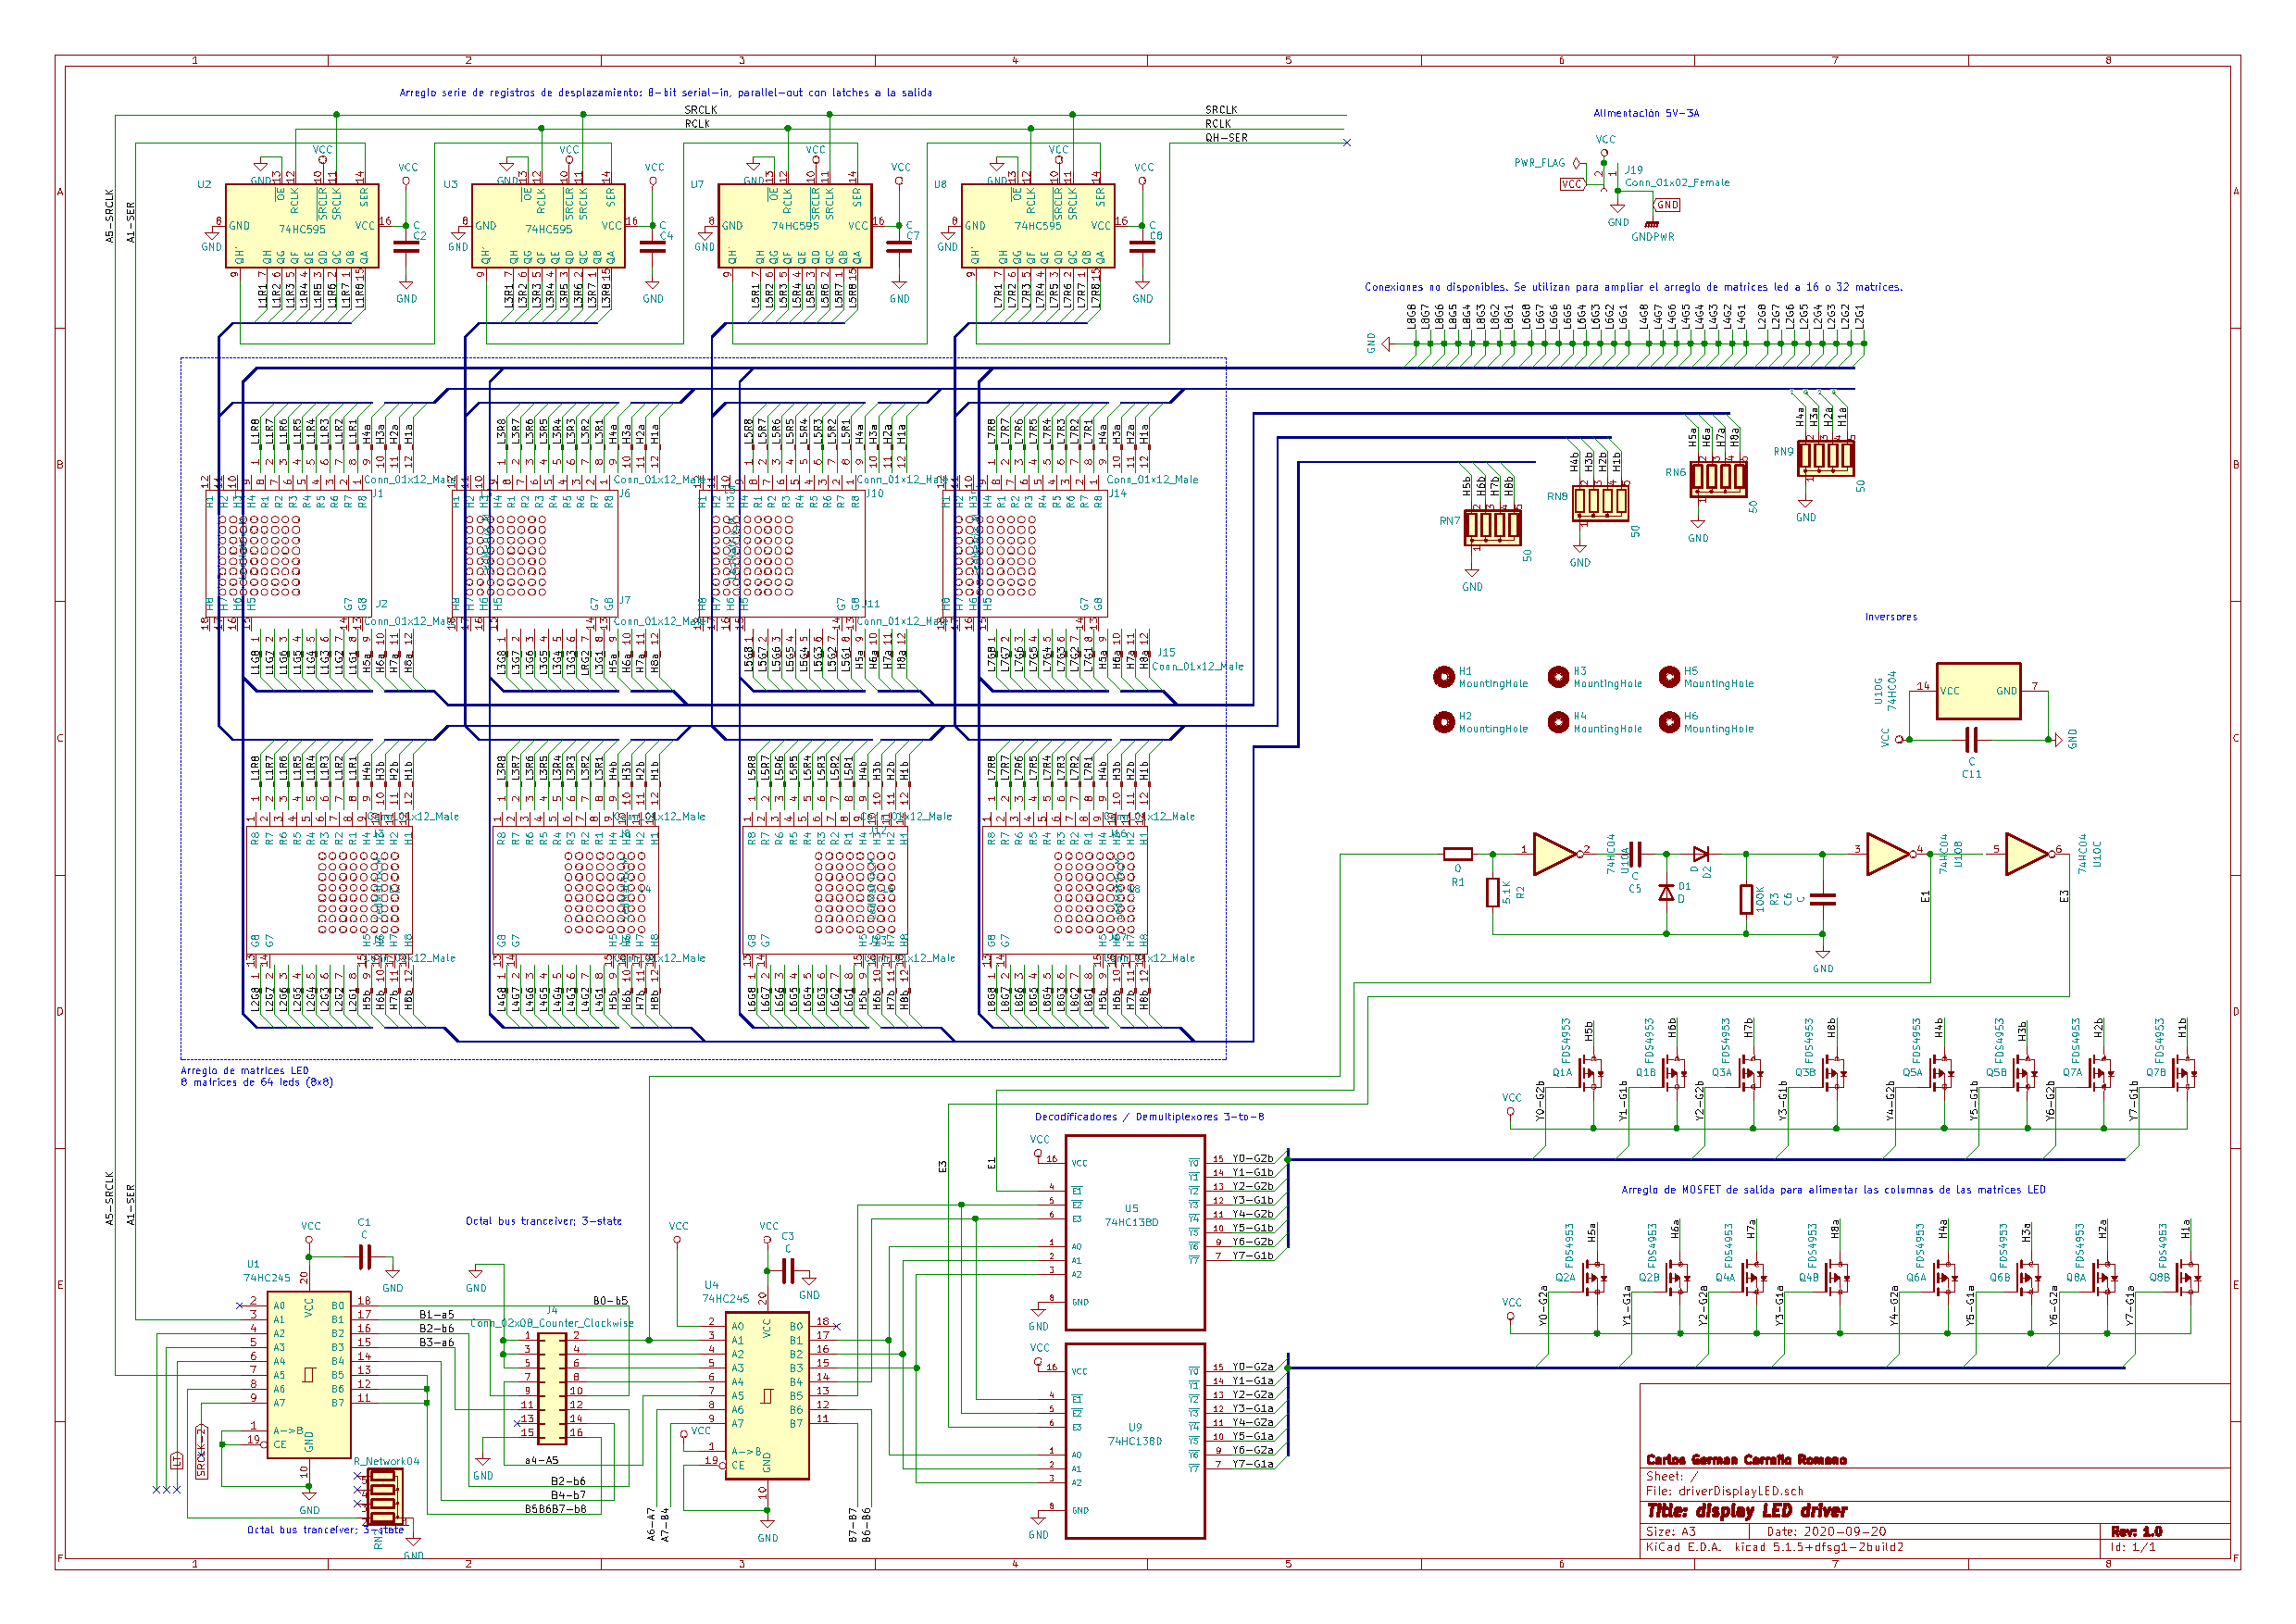
\includegraphics[width=1.66\textwidth, angle=90]{./Figures/output.driverLED.pdf}
	\caption{Circuito esquemático de la placa controladora de los carteles de matriz LED.}
	\label{fig:schDriverLED}
\end{figure}

La pieza de software desarrollada para el control del display led es un objeto activo consistente con el resto del sistema. El diagrama de la máquina de estados asociada se presenta en la figura \ref{fig:fsmDisplayLED}. \\

\begin{figure}[ht]
	\centering
	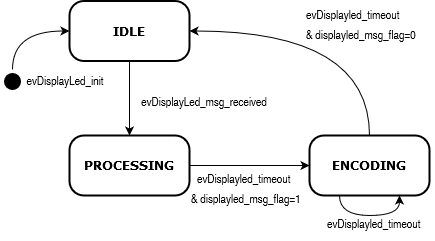
\includegraphics[width=0.66\textwidth]{./Figures/FSMdisplayLed.png}
	\caption{Diagrama de estados para la máquina de estados del display Led.}
	\label{fig:fsmDisplayLED}
\end{figure}


Se pueden distinguir tres estados, cada uno con un handler asociado. En el siguiente fragmento de código se presenta la especificación de la máquina de estados del display led. \\


\begin{lstlisting}[
	language=C, 
	backgroundcolor=\color{mygray},
	caption=	{Display Led state machine definition},
	captionpos=b]
sStateMachine_displayLed fsmDisplayLed[] = 
{
    {STATE_DISPLAYLED_INIT, evDisplayled_init, displayled_initHandler},
    {STATE_DISPLAYLED_IDLE, evDisplayled_msg_received, displayled_idleHandler},
    {STATE_DISPLAYLED_PROCESSING, evDisplayled_timeout, displayled_procHandler},
    {STATE_DISPLAYLED_ENCODING, evDisplayled_timeout, displayled_dataHandler}
};
\end{lstlisting}
\label{code:fsmDisplay}



\begin{lstlisting}[
	language=C, 
	backgroundcolor=\color{mygray},
	caption=	{Código fuente del handler de procesamiento del display led.},
	captionpos=b]

eSystemState_displayLed     displayled_procHandler(void){

    char *str1=messages[displayled_msg_idx];

    uint8_t str1_len=strlen(str1);
    uint8_t buffer_size=str1_len*CHAR_LENGTH;
    uint8_t buffer[buffer_size];

    string_read_to_8x8_bytes_out(str1,str1_len,buffer);

    int n=CHAR_LENGTH; 
    int m=str1_len;
    int p=DISPLAYLED_ROWS;
    int q=DISPLAYLED_COLS;

    int displayled_size = p*q;

    uint8_t B[displayled_size];
    for(int i=0; i<displayled_size;i++)
    B[i]=0;

    reshape_to_display(buffer, displayled_buffer, buffer_size, displayled_size);

    displayled_msg_idx++;
    displayled_msg_idx%=MESSAGES_TOTAL_NUMBER;
    displayled_msg_flag=0;

    return STATE_DISPLAYLED_ENCODING;
}

\end{lstlisting}

El estado 'STATE\_DISPLAYLED\_PROCESSING' ejecuta el handler  'displayled\_procHandler()' encargado de recibir mensajes externos en formato string (char*). Este implementa un pipeline de procesamiento para transformar strings en matrices de enteros de 8 bits.

\begin{figure}[ht]
	\centering
	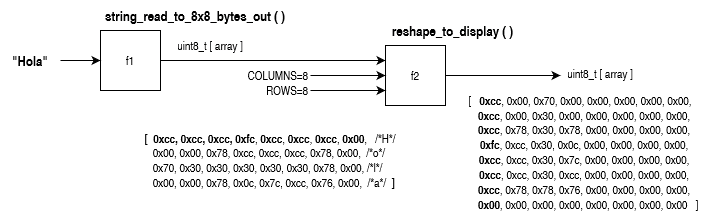
\includegraphics[width=1\textwidth]{./Figures/pipelineDataEncoding.png}
	\caption{Lógica de procesamiento de datos para visualizar en el display.}
	\label{fig:displayDataLogic}
\end{figure}


\begin{lstlisting}[
	language=C, 
	backgroundcolor=\color{mygray},
	caption=	{Código fuente del handler de encoding del display Led.},
	captionpos=b]
	
eSystemState_displayLed     displayled_dataHandler(void){

    uint8_t data_8b;
    bool_t  value;

    displayled_timer_cnt--;
    if(!displayled_timer_cnt){
        displayled_msg_flag=0;
        return STATE_DISPLAYLED_IDLE;
    };    

    for(int i=0; i<displayled_size; i++){
        
        data_8b = displayled_buffer[i];
        
        for(int j=0; j<8; j++){
            
            // displayled_data 
            value = (((data_8b << j ) & 0x80 ) == 0) ? 1 : 0;
            printf("%d",value);
            gpioWrite(displayled_panel_1, value);
            gpioWrite(displayled_panel_2, value);
            
            // displayled_clock 
            gpioWrite(displayled_clk, ON);
            gpioWrite(displayled_clk, OFF);
        }
        
        if(i%DISPLAYLED_COLS==0){

            // displayled_latch 
            printf("\r\n");
            gpioWrite(displayled_latch, ON);
            gpioWrite(displayled_latch, OFF);
            
            // displayled_row_scanning
            displayled_deco_cnt++;
            displayled_deco_cnt%=DISPLAYLED_ROWS;
            if((displayled_deco_cnt%1)==0){ 
            		gpioToggle(displayled_deco_A0); }
            if((displayled_deco_cnt%2)==0){ 
            		gpioToggle(displayled_deco_A1); }
            if((displayled_deco_cnt%4)==0){ 
            		gpioToggle(displayled_deco_A2); }
            if((displayled_deco_cnt%8)==0){ 
            		gpioToggle(displayled_deco_A3); }
        }
    }
    
    return STATE_DISPLAYLED_ENCODING;
}

\end{lstlisting}
